%%%%%%%%%%%%%%%%%%%%%%%%%%%%%%%%%%%%%%%%%
% Structured General Purpose Assignment
% LaTeX Template
%
% This template has been downloaded from:
% http://www.latextemplates.com
%
% Original author:
% Ted Pavlic (http://www.tedpavlic.com)
%
% Note:
% The \lipsum[#] commands throughout this template generate dummy text
% to fill the template out. These commands should all be removed when 
% writing assignment content.
%
%%%%%%%%%%%%%%%%%%%%%%%%%%%%%%%%%%%%%%%%%

\documentclass{article}

\usepackage{fancyhdr} % Required for custom headers
\usepackage{lastpage} % Required to determine the last page for the footer
\usepackage{extramarks} % Required for headers and footers
\usepackage{graphicx} % Required to insert images
\usepackage[utf8]{inputenc}

% Margins
\topmargin=-0.45in
\evensidemargin=0in
\oddsidemargin=0in
\textwidth=6.5in
\textheight=9.0in
\headsep=0.25in 

\linespread{1.1} % Line spacing



\setlength\parindent{0pt} % Removes all indentation from paragraphs

%----------------------------------------------------------------------------------------
%	DOCUMENT STRUCTURE COMMANDS
%	Skip this unless you know what you're doing
%----------------------------------------------------------------------------------------

% Header and footer for when a page split occurs within a problem environment
\newcommand{\enterProblemHeader}[1]{
\nobreak\extramarks{#1}{#1 continued on next page\ldots}\nobreak
\nobreak\extramarks{#1 (continued)}{#1 continued on next page\ldots}\nobreak
}

% Header and footer for when a page split occurs between problem environments
\newcommand{\exitProblemHeader}[1]{
\nobreak\extramarks{#1 (continued)}{#1 continued on next page\ldots}\nobreak
\nobreak\extramarks{#1}{}\nobreak
}

\setcounter{secnumdepth}{0} % Removes default section numbers
\newcounter{homeworkProblemCounter} % Creates a counter to keep track of the number of problems

%----------------------------------------------------------------------------------------
%	NAME AND CLASS SECTION
%----------------------------------------------------------------------------------------

\newcommand{\lessonNumber}[1]{Lezione\ \##1} % Assignment title
\newcommand{\lessonDate}[4]{#1,\ #2\ #3\ #4} % Due date
\newcommand{\lessonCourse}[1]{#1} % Course/class
\newcommand{\lessonTime}[1]{#1} % Class/lecture time
\newcommand{\lessonTeacher}[1]{#1} % Teacher/lecturer
\newcommand{\lessonAuthor}[1]{#1} % Your name
\begin{document}
\section{Ingegneria dei requisiti(8)}

L'attività di \textbf{analisi dei requisiti} è importantissima, comporta molte competenze ed è complessa, per cui viene chiamata \textbf{Ingegneria dei requisiti}. Un requisito può essere visto da due lati:

\begin{itemize}

	\item \textbf{Vista cliente:} qual'è il bisogno da soddisfare;
	\item \textbf{Vista fornitore:} come deve essere la soluzione del bisogno.

\end{itemize}

Dovrò prima interrogare gli stakeholders e poi chiedermi cosa serve a me per soddisfare quei requisiti. Quando queste due cose sono soddisfatte avrò soddisfatto il \textbf{requisito utente}. Sui requisiti si effettua \textit{breakdown}, spezzamento, perchè rende più facile verificare che siano soddisfatti.\\

Dei processi di supporto al ciclo di vita sono:
\begin{itemize}

	\item La \textbf{Verifica:} faccio in modo che tutte le attività assegnate introducano la più piccola possibilità di errore, rivolta principalmente ai processi (modo di lavorare);
	\item la \textbf{Validazione:} accertare che il prodotto realizzato corrisponda alle attese.

\end{itemize}

Questi due processi formano la \textbf{qualifica}.

Si lavora sempre secondo regole di procedura. Devono esistere delle regole prima di iniziare il lavoro. Avremo alla fine specializzato un prodotto che soddisfa i requisiti iniziali e le sue aspettative. Un lavoro \textbf{verificato} è un lavoro fatto nel modo giusto e secondo le regole date. \\

Molti dei sistemi al giorno d'oggi sono detti \textbf{socio-tecnici}, hanno come dato rilevante l'elemento \textbf{umano}, che è come la persona userà quel prodotto. Chiedersi che ruolo ha l'utente umano nel sistema è parte fondamentale dell'AR. In ogni sistema organizzato c'è uno \textit{sportello} rivolto all'umano; molto spesso si chiama \textit{front office} (interfaccia utente). L'opposizione è il \textit{back office} in cui si prepara ciò che andrà al front office (es. database). Devo capire entrambe queste parti per realizzare un sistema socio-tecnico. E' molto raro progettare un sistema esclusivamente tecnico. Ci sono due fasi:

\begin{itemize}

	\item \textbf{Analisi:} analisi dei bisogni e delle fonti, classificazione dei requisiti, visione UC, confronto con le fonti(committente, sottofornitori);
	\item \textbf{Validazione:} successiva all'Analisi, predispone la revisione interna/esterna, di prove e dimostrazioni.

\end{itemize}

In questa fase i processi coinvolti sono la \textbf{Documentazione} (studio di fattibilità, analisi dei requisiti) e la \textbf{Gestione e manutenzione dei prodotti} (tracciamento dei requisiti, impostazione e gestione della configurazione, gestione dei cambiamenti).\\
Questo tipo di analisi dei requisiti da luogo a un ciclo di vita simile, modello incrementale:\\
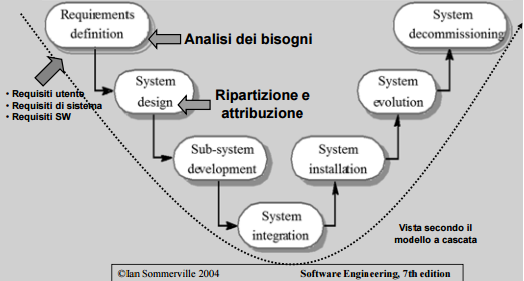
\includegraphics[width=0.75\columnwidth]{img1}
\\
I prodotti attesi alla fine di questa fase sono molteplici:

\begin{itemize}
	\item Dall'analisi dei bisogni e delle fonti:
	\begin{itemize}
		\item \textbf{Definizione dei requisiti:} genera il capitolato d'appalto(unico di responsabilità del cliente, definisce i requisiti)
		\item \textbf{Specifica dei requisiti:} genera lo studio di fattibilità (All'interno si valutano rischi, costi e benefici per decidere se procedere) e l'analisi dei requisiti, serve a valutare rischi (individuazione dei rischi), costi e benefici per poi decidere se procedere
	\end{itemize}
	\item Dalla ripartizione dei requisiti
	\begin{itemize}
		\item \textbf{Modellazione concettuale del sistema SW:} genera la specifica tecnica (caratterizzazione architetturale dei componenti)
	\end{itemize}
\end{itemize}

Per produrli si può  ricorrere a due tipi di approccio \textbf{Approccio Funzionale} \textbf{Approccio Object-Oriented}

Un ulteriore passo sarà quello della classificazione dei requisiti trovati:
\begin{itemize}
	\item \textbf{Attributi di prodotto:} definiscono le caratteristiche richieste al sistema, esprimono \textit{requisiti funzionali, prestazionali e quantitativi} 
	\item \textbf{Attributi di processo:} pongono vincoli sui processi impiegati nel progetto, esprimono \textit{ulteriori requisiti extra-funzionali}
\end{itemize}


Sicuramente i requisiti devono essere verificabili, chi impone un requisito teoricamente deve avere anche idea di come accertarne il soddisfacimento, vediamo per i vari tipi di requisiti una linea guida per verificarli, prima di tutto ci sono due macro categorie che sono gli attributi di prodotto (definiscono le caratteristiche richieste al sistema) e quelli di processo (pongono vincoli sui processi impiegati nel sistema):

\begin{itemize}
	\item Requisiti funzionali: test, dimostrazione formale, revisione;
	\item Requisiti prestazionali: misurazione;
	\item Requisiti qualitativi: verifica ad hoc;
	\item Requisiti dichiarativi: revisione.
\end{itemize}
in oltre tutti questi tipi di requisiti hanno diversa utilità strategica, possono essere:
\begin{itemize}
	\item \textbf{Obbligatori:} irrinunciabili per qualsiasi stakeholder;
	\item \textbf{Desiderabili:} non strettamente necessari ma di valore aggiunto riconoscibile;
	\item \textbf{Opzionali:} relativamente utili, contrattabili in seguito.
\end{itemize}

L'interesse di un fornitore è \textbf{negoziare} questi requisiti. A noi sta il compito di classificare in modo elastico. I requisiti non devono essere in contraddizione tra loro, non devono essere mai in conflitto o sovrapposti. I requisiti nascono scritti in un linguaggio naturale, (\textit{i capitolati}) e noi vogliamo portarci in un linguaggio che sia il più vicino possibile ad automi. Cercheremo tecniche che rendono il più possibile automatico ciò che facciamo (es. UML o tabelle).\\

\textbf{IEE 830-1998} è un documento che descrive le pratiche raccomandate per scrivere la specifica dei requisiti. Ci sono 8 proprietà fondamentali:

\begin{enumerate}

	\item \textbf{Unambigous:} mai alcuna incertezza su che cosa significano;
	\item \textbf{Correct:} non deve nascere sbagliato perchè fa danni;
	\item \textbf{Completi} ;
	\item \textbf{Verifiable:} a basso costo;
	\item \textbf{Consistence:} non posso chiedere una cosa e il suo contrario;
	\item \textbf{Modifiable:} serve una tecnica che renda modificabile l'insieme dei requisiti. Sui requisiti devo poter aggiungere, togliere, cercare, aggiornare: operazioni tipiche da basi di dati;
	\item \textbf{Traceable:} deve essere univocamente identificabile;
	\item \textbf{Ranked:} per rilevanza.

\end{enumerate}

\textbf{Verifica dei requisiti}
Deve essere eseguita su un documento organizzato. Tecnica di ricerca \textit{a pettine}, \textbf{walkthrough}, tecnica completamente manuale, una ricerca a largo spettro; lo si fa quando non si sa esattamente cosa cercare; tecnica dell'\textbf{ispezione}, in cui c'è una lettura mirata e strutturata; questa tecnica è molto più automatizzabile. 

Facendo walkthrough impariamo e sviluppiamo tecniche per fare ispezione. Sui requisiti devo poter fare una buona identificazione e classificazione. Dentro un progetto tutto rimanda ai requisiti, tutto è sempre in una forma tracciabile e riconducibile al \textit{perchè è lì}, questo deve essere fatto attraverso procedure e automatizzazioni.\\

\textbf{SEMAT}, nella struttura c'è una progressione di stati molto utili da analizzare. I requisiti hanno un ciclo di vita proprio che passa attraverso 6 stati, ciascuno con delle dipendenze.
\begin{enumerate}
	\item \textbf{Conceived:} (concepito), si vede un'opportunità nel fare le cose e i committenti sono identificati. \textbf{Bounded}, i requisiti sono su un recinto e potrò ragionare macroscopicamente di fattibilità;
	\item \textbf{Coherent:} quando i requisiti sono classificati e quelli chiari sono distinti;
	\item \textbf{Acceptable:} diventa un punto dal quale avanzare e dal quale non vorremmo mai retrocedere, \textit{Base line};
	\item \textbf{Addressed:} i requisiti sono collocati, ho delle soluzioni specifiche e il prodotto che sto facendo soddisfa i requisiti. Questo stato lo raggiungiamo prima del collaudo;
	\item \textbf{Fullfilled:} in cui ``le cose sono soddisfatte'', stato dell'accattazione. Le transizioni sono più vicine nel tempo nella parte iniziale
\end{enumerate} 

\end{document}